%!TEX root = ../template.tex
%%%%%%%%%%%%%%%%%%%%%%%%%%%%%%%%%%%%%%%%%%%%%%%%%%%%%%%%%%%%%%%%%%%%
%% chapter4.tex
%% NOVA thesis document file
%%
%% Chapter with lots of dummy text
%%%%%%%%%%%%%%%%%%%%%%%%%%%%%%%%%%%%%%%%%%%%%%%%%%%%%%%%%%%%%%%%%%%%

\typeout{NT FILE chapter4.tex}%

\chapter{Design}
\label{cha:test}

In this chapter, we present the design of our system and discuss alternatives to the decisions we took in our implementation.
A modular approach was adopted to construct the system;
each module is entirely independent, making it easy to interchange alternative approaches.
We dedicate the first half of this chapter to define the goals that guided the design of system,
the remainder of the chapter will be used to discuss each design aspect in turn.

\section{Discussion} % (fold)
\label{sec:discussion}

Recall that the problem we are trying to solve is how to make the process of updating contracts in
microservice-based systems more robust, in the sense that it should be harder to deploy a service that could
potentially break the system soundness.
There are many approaches to solve this problem, each with its own set of compromises.
The goals that informed our decisions, are outlined below by their priority:

\begin{itemize}
    \item Supporting all types of contract changes
    \item Integration with existing tools and workflows
    \item Minimize conception and maintenance effort
    \item Automatic validation of the safety of deployment operations
    \item Consumers and producers are unaware to the presence of adapters
    \item Transactionless deployment and upgrade of service contracts
    \item No downtime when upgrading service contracts
    \item No overhead when services communicate using the same contract version
\end{itemize}

Four principles were considered when evaluating each approach:
\textbf{Flexibility} the applicability of the approach under diverse scenarios;
\textbf{Effectiveness} the efficiency of an approach at solving a problem;
\textbf{Utility} the effort required to adopt and maintain the approach;
\textbf{Performance} the overhead associated with approach;

In the prototype's design, we prioritized utility above performance because,
in the common case, each service will communicate via up-to-date contracts and
because the effort associated with adopting an approach will be proportional to the complexity and size of a contract and its evolution,
whereas the performance overhead will remain mostly static under diverse contract changes, as it is largely attributable to communication costs.
We prioritized flexibility and effectiveness above other principles because if an approach isn't applicable or effective under a scenario,
then it will be necessary to adopt hybrid solutions, which will have a detrimental effect on the utility of the entire solution.

\section{Design Aspects} % (fold)
\label{sec:design_aspects}

\subsection{Communication protocol} % (fold)
\label{sec:communication_protocol}

The communication protocol defines the syntax, semantics and synchronization of communication between microservices.
Our choice in the communication protocol is bounded by the adopted communication strategy between microservices, orchestration or choreography.
Orchestration relies on request-response protocols while choreography relies on event-driven protocols.

\paragraph{Approach}
Most applications require a web presence and microservice systems that
rely on choreography still require the HTTP request-response protocol to have a web presence,
for this reason we chose to design our system around the orchestration pattern and the HTTP protocol.

\paragraph{Alternative}
Other event-driven and request-response protocols, such as RPC, have a simplified
syntax, and there are already a number of tools that support the evolution of schemas
under these protocols, albeit with some limitations.

\subsection{Contract Specification} % (fold)
\label{sec:contract_specification}

It is required that each microservice’s interface be
described in a high-level language which abstracts away implementation details, because it is common
for microservices to be implemented under different frameworks and programming languages.
We use these interface specifications to clearly define and document the procedures of a service and its consumed resources and requirements.

\paragraph{Approach}
Because most API definition frameworks do not allow the explicit declaration of dependencies and requirements of a service,
contracts are represented in two distinct manifest files, one defines the procedures of a service, and the other dictates its consumed resources and requirements.
The definition of a service dependencies and requirements has three benefits: it allows a deployment to be validated and blocked if the corresponding requirements are not met within the system,
it allows for the automatic removal of un-utilized adapters without developer intervention,
and it allows developers to clearly see the impact of a contract change on the entire system, as well as the effort required to support the change.

\paragraph{Alternative}
Services dependencies can be determined indirectly by automatically inspecting request logs between services.
The advantage of this approach is the reduced documentation effort, but it comes at a cost because
it is no longer possible to validate the safety of service deployments;
it is only possible to validate the safety of the removal of services.
Un-needed adapters would also have to be removed manually by developers or through an automated inactivity-based warning system.

\subsection{Compatibility Verification} % (fold)
\label{sec:compatibility_verification}

Intuitively, compatibility verification determines whether
all the edited elements in a producer service contract are compatible with the ones effectively
used by the consumer services, and whether the new contract requirements are met
by the system’s existing resources.

\paragraph{Approach}
The verification procedure examines both the producer contract and all consumer references to determine the safety of a deployment operation.
Edited elements are considered compatible if the information supplied by prior elements is sufficient to meet the edited elements parameters.
Contract requirements are fulfilled if there are enough computational resources to accommodate the service and if all the
service dependencies are available and reachable in the system.

\paragraph{Alternative}
Instead of determining if a new contract version is compatible with all consumer references,
we evaluate only whether the new contract is compatible with the prior versions that are still in use.
If a new contract is missing a capability that was present in a prior version,
the developers will need to verify if the capability is not being consumed
and mark it as obsolete in the evolution manifest for the contract to be considered safe.
This approach has the advantage of streamlining the verification process by eliminating the
need for all contracts to be accessible by machine code in a standardized fashion.
The downside is that it introduces human error in the verification of un-utilized service capabilities.

\subsection{Tools} % (fold)
\label{sec:tools}

In distributed systems there is a lack of tools
comparable to those used in centralized systems, for visualizing the impact of a change and effort required to implement it.
In this section, we discuss how such tools could be implemented.

\paragraph{Approach}
Since all service contracts declare their dependencies on other services procedures, determining the impact of change in a procedure is as simple as
looping over all active services contracts and verifying whether the changed procedure is being consumed.
Then, using this information, a report indicating all affected services and other metadata may be created.
We store service contracts in the same repository as the service code, with semantic versioning, where
each major version represents incompatible contract changes and minor versions represent backward compatible contract changes.
To discover the active services, we run a query against the container orchestration tool, which returns the deployed services.
A tool like this may be easily created in a bash script and its results shown in an IDE.
If kubernetes and git are utilized, the active services may be queried with the \textbf{kubectl} command line tool,
and the service contracts can be fetched using the git repository urls and standard naming convention for the service contracts.

\paragraph{Alternative}
The information about the active services and individual service contract can be translated into an ontology language and hosted in a centralized registry.
The main advantage of this approach is that allows us to easily integrate the registry with a reasoning system capable of performing deductive inferences over the service's data, such as
inferring the consumers of a service procedure given the procedure and service name or generating a graph structure that maps all participating services dependencies.
This approach would allow us to obtain richer data and reduce the burden of the development of sophisticated tools.
The drawback is that the update of some information might require the use of distribute transactions to avoid incoherent data,
for example renewing the services that are participating in the system.

\subsection{Evolution Specification} % (fold)
\label{sec:evolution_specification}

It is not always possible to implicitly deduce the evolutions in a contract when comparing a new version to a prior version.
For example, renaming one field \textbf{A->B} is indistinguishable, from inserting a new field \textbf{B} and removing another field of the same type \textbf{A}.
The developer must declare which evolution occurred explicitly.

\paragraph{Approach}
The evolutions are specified in a manifest file, complete with its own syntax and rules,
which outlines how to adapt calls between two versions of the contract.
In this file all mappings between elements in each version are explicitly defined.
A mapping for one element can fall into one of three types:
\begin{itemize}
    \item \textbf{Default value}: The developer provides a default value for the element.
    This mapping is only valid if the default value has the same type and format as the element.
    \item \textbf{Link}: The developer indicates that element X on the previous contract is equivalent to element Y in the new contract.
    This mapping is only valid if the two elements have the same type and format.
    \item \textbf{Function}: The developer applies a function over Xn elements of previous contract and indicates that the result of the function is equivalent to element Y in the new contract.
    This mapping is only valid if the function's output type and format are equal to element Y and if the function's arguments match the type and format of the provided Xn elements.
\end{itemize}
Renamed fields in contracts are supported with the use of links.
The addition of new fields in contracts is supported with the use of default values.
Complex contract changes, such as changing the format of a date are supported with the use of functions.

\paragraph{Alternative}
The evolution specification is defined in conjunction with the contract specification.
Most web API specification languages already support default values and name aliases.
With these two features it would be possible
to support the following contract evolutions: renamed fields, addition of fields and removal of fields.
For simple contract this alternative can seem appealing, but as the number of revisions and consumers in prior versions rises, this solution becomes impractical.
This approach clutters the contract with information that is irrelevant to consumers, and makes the specification of complex contract changes more cumbersome.

\subsection{Adapter Location} % (fold)
\label{sec:adapter_location}

The adaptation of messages is supported at runtime by a generated proxy component
that dynamically adapts the data exchanged between services.
The adapter can be deployed and intercept messages in different points through the exchange.

\paragraph{Approach}
The adapter is installed in a separate container but on the same node as the service container.
Consumers direct their requests based on the expected version of the service using a routing rule.
If the expected version matches the current service version, the request is answered directly by the service;
otherwise, the request is redirected through the adapter.
Since the adapter and the service are in the same node, the communication cost is expected to be comparable to the cost of inter-process message passing.
The main benefit of this approach is that the adapter can be deployed alongside the service,
which circumvents distributed transactions in deployments,
because container orchestrations tools such as kubernetes allow the deployment of closely related containers as atomic units known as "pods".

\paragraph{Alternative A.}
The adapter code is embed in the service implementation.
This approach is expected to have higher performance than the previous approach since
the adapter would use function calls instead of inter-process calls, and because message serialization and de-serialization would be unnecessary.
The downside of this approach is that it would entail the modification of the service's code, which is problematic because each service can be implemented in a different framework and programming language.

\paragraph{Alternative B.}
The adapter is installed in the nodes of all the service consumers.
This approach is problematic because a service upgrade would entail the re-deployment of all consumers.
If one of the re-deployments fails, the entire service upgrade would have to be cancelled;
this is only achievable with the use of distributed transactions, which are inherently complex.
The re-deployment of adapters can be avoided with the use of mobile code that is provided by the service in a dedicated endpoint.
This could be accomplished in Java with the use of network class loaders.
We find this approach ineffective because it provides no benefits and requires more resources than alternative approaches since,
instead of one adapter, we would need N adapters, one for of the service consumers.

\subsection{Adapter Polymorphism} % (fold)
\label{sec:adapter_polymorphism}

The adapter can have a generic implementation that is able to adapt messages from any service, or it can
have a direct implementation that can only manage the exchange of messages for one service.

\paragraph{Approach}
The adapter implementation is derived from a template implementation,
that is completed with the substitution of template variables with code generated from a single evolution specification manifest file.
The advantage of this approach is that the implementation will be more performant than generic approaches.

\paragraph{Alternative}
The adapter haves a generic implementation and determines how to adapt messages by inspecting specialized headers in the
message that indicate the message type, service and version and by consulting the corresponding evolution manifest.
The advantage of this approach is that a single adapter can convert messages from any service as long as the evolution manifests are supplied to the adapter beforehand.
This approach will consume fewer computational resources, in scenarios where the number of messages that require adaptation is low and uniformly distributed across all services,
because a single adapter can handle the load of all requests, whereas the other approach requires one adapter per service.
The downside of this approach is that it requires modifying the service's implementation to add the message headers.
The mentioned benefit is obviously lost if the adapter is embedded in every service's node.

\subsection{Adapter Management} % (fold)
\label{sec:adapter_management}

The operations of contract compatibility verification, adapter generation, deployment, and removal should be automated.
In this section, we discuss how to integrate these operations with the more common operations of service deployment and upgrade.

\paragraph{Approach}
We propose to include these operations in stages of continuous deployment pipelines.
The operations of compatibility verification and adapter generation are supported by executables in container images that run as pipeline jobs.
The verification of contract compatibility should take place prior to the packaging stage.
The generation of the adapter implementation may be conducted after the unit test stage but before acceptance test stage,
the adapter should be tested integration and stress tests.
Adapters could be deployed and removed in tandem with service deployments, in the last stage of the pipeline.

\begin{figure}[htbp]
    \centering
    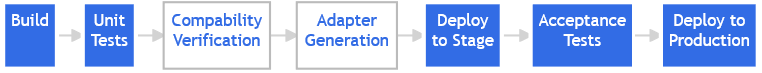
\includegraphics[height=0.56in]{CD}
    \label{fig:gantt}
\end{figure}